\documentclass[../physical_computing.tex]{subfiles}

\begin{document}

\chapter{Sequential Circuits}
\label{sec:registers}

\section{Motivation}
\label{sec:motivate_sequential}

In chapter \ref{sec:logic_and_integers} we investigated logic gates
and more general devices possessing truth tables. We can imagine 
that a great many problems can be solved purely using logic; given enough input data bits, and enough logic gates, a configuration of 
logic gates could be found that could produce a correct result. 
However, there certainly exist questions that cannot be answered by logic alone. For example, how long is it between flashes of that 
light? That one can't be done with a pure logic circuit because logic alone cannot wait or measure time. Or how about solving the equation $\tan(x)=x$?. Or how about any circuit that executes tasks in
responds to commands issued by humans?

In these cases, we are going to need more elements in our armoury than just logic gates. The thing that these examples have in common is that solving them requires a circuit that can work with intermediate results. In the first case, if you have an oscillator, you can detect its pulses, and each time you detect a pulse, you can increment a counter, so long as you have some way of memorising where the count has got to. You can then gate the counter to start when one light pulse is detected and stop on the detection of the next one. In the second case, there are many numerical methods of solving nonlinear equations like $\tan(x)=x$, such as the Newton Raphson method. These methods rely on starting at some initial guess, then using an iterative procedure to converge on the right answer, within some required tolerance. But in order to work, these techniques need to store intermediate results, and logic gates cannot store anything. In the final
case, the circuit has to ask for a command, wait for it to be entered, memorise it, act on it, and then perhaps ask for another command. There are plenty of intermediate results and some waiting to do.

\section{Trouble with logic}
\label{sec:trouble}

As a first step in seeing how we might introduce some of the necessary elements into our circuit, let's consider a troublesome logical
circuit, shown in various representations in Figure 
\ref{fig:self_contradicting_logic}.

\begin{figure}[htbp]
    \centering
    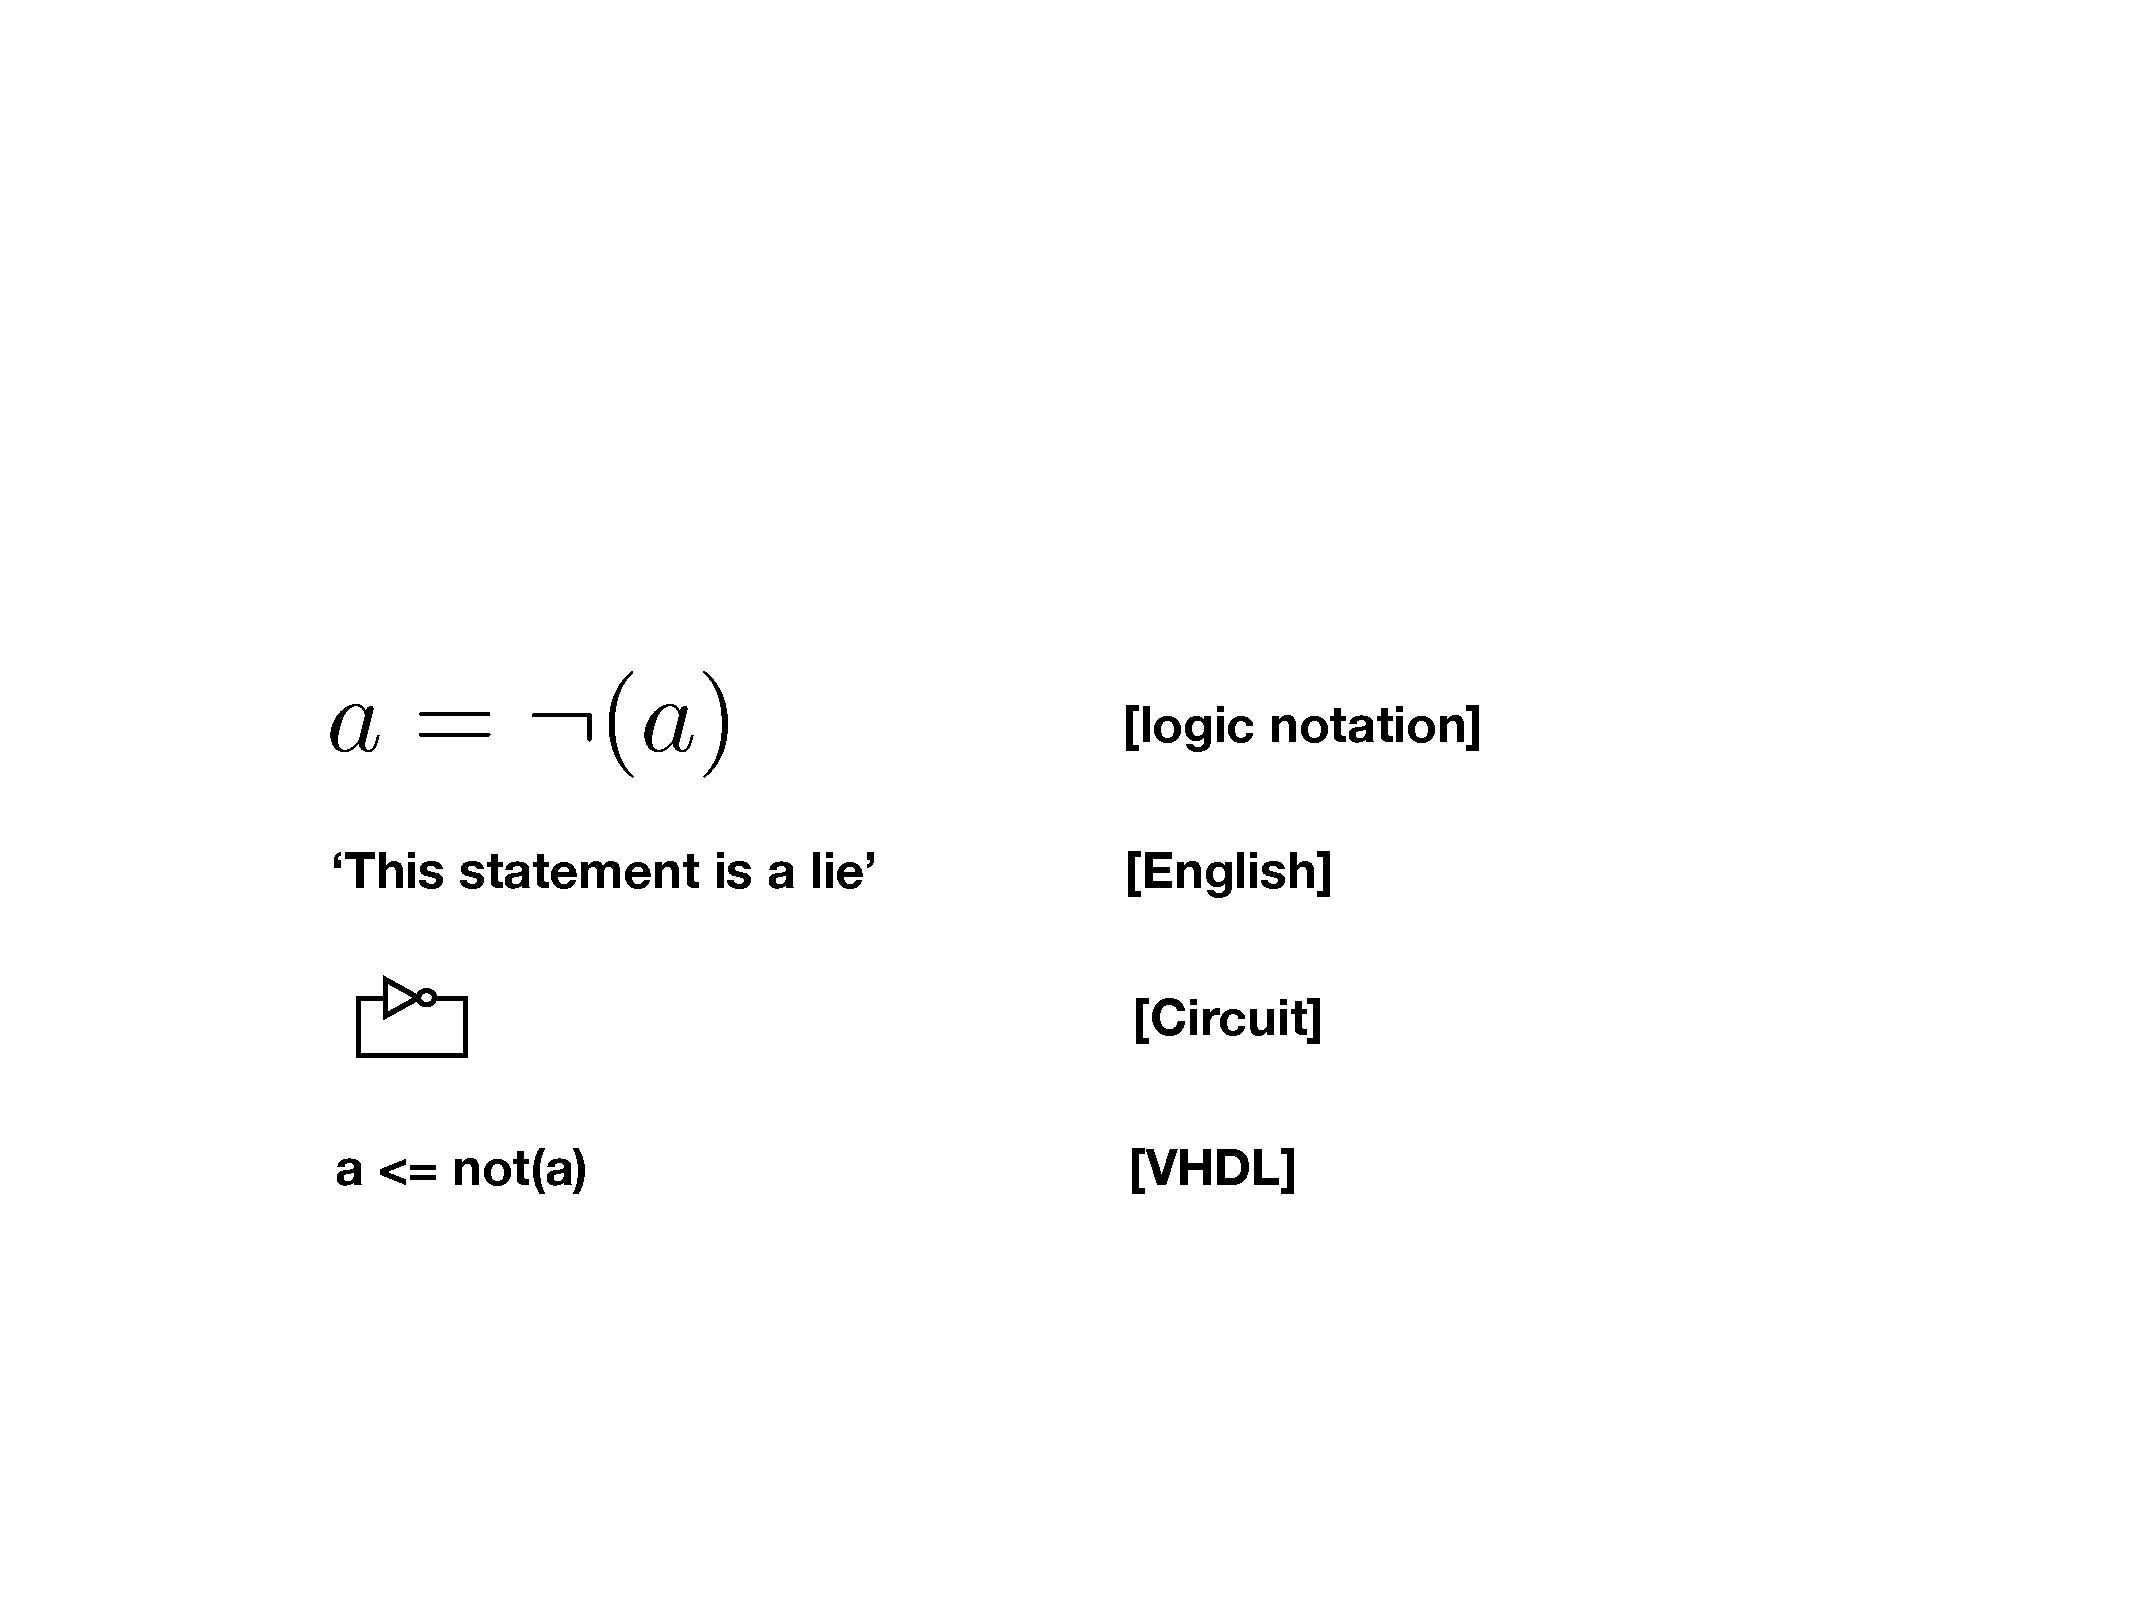
\includegraphics[width=0.5\textwidth]
    {figures/self_contradicting_logic.pdf}
    \caption{An internally inconsistent circuit in various
    representations.}
    \label{fig:self_contradicting_logic}
\end{figure}

This is the kind of statement that Kurt G\"odel was worried about
in connection with the programme of building a complete and self-consistent logical framework for mathematics \cite{Hofstadter:99665,Smullyan}. You can 
immediately see the problem with it - if it is true that the
statement is a lie, then it must be false, and there is a 
contradiction.

\section{Oscillators}
\label{sec:oscillators}

In fact, this statement is rather close to the science of 
oscillators, as you can see by inserting the simple words,
`a moment ago'. If you say 'a moment ago, this statement was
a lie', then it's fine because a moment ago it can have been 
a lie, so it is now a true statement that it was a lie
before. A moment from now, it will be false that a moment ago
the statement was a lie, actually it was true then, and so forth.
In science terms, if we insert a time delay in the loop with 
the not gate, there is a consistent signal that can exist
indefinitely in the circuit.
In Figure \ref{fig:oscillator_logic} a $\rm 1\,ns$
time delay has been inserted, resulting in a $\rm 2\,ns$ period
square wave oscillator.

\begin{figure}[htbp]
    \centering
    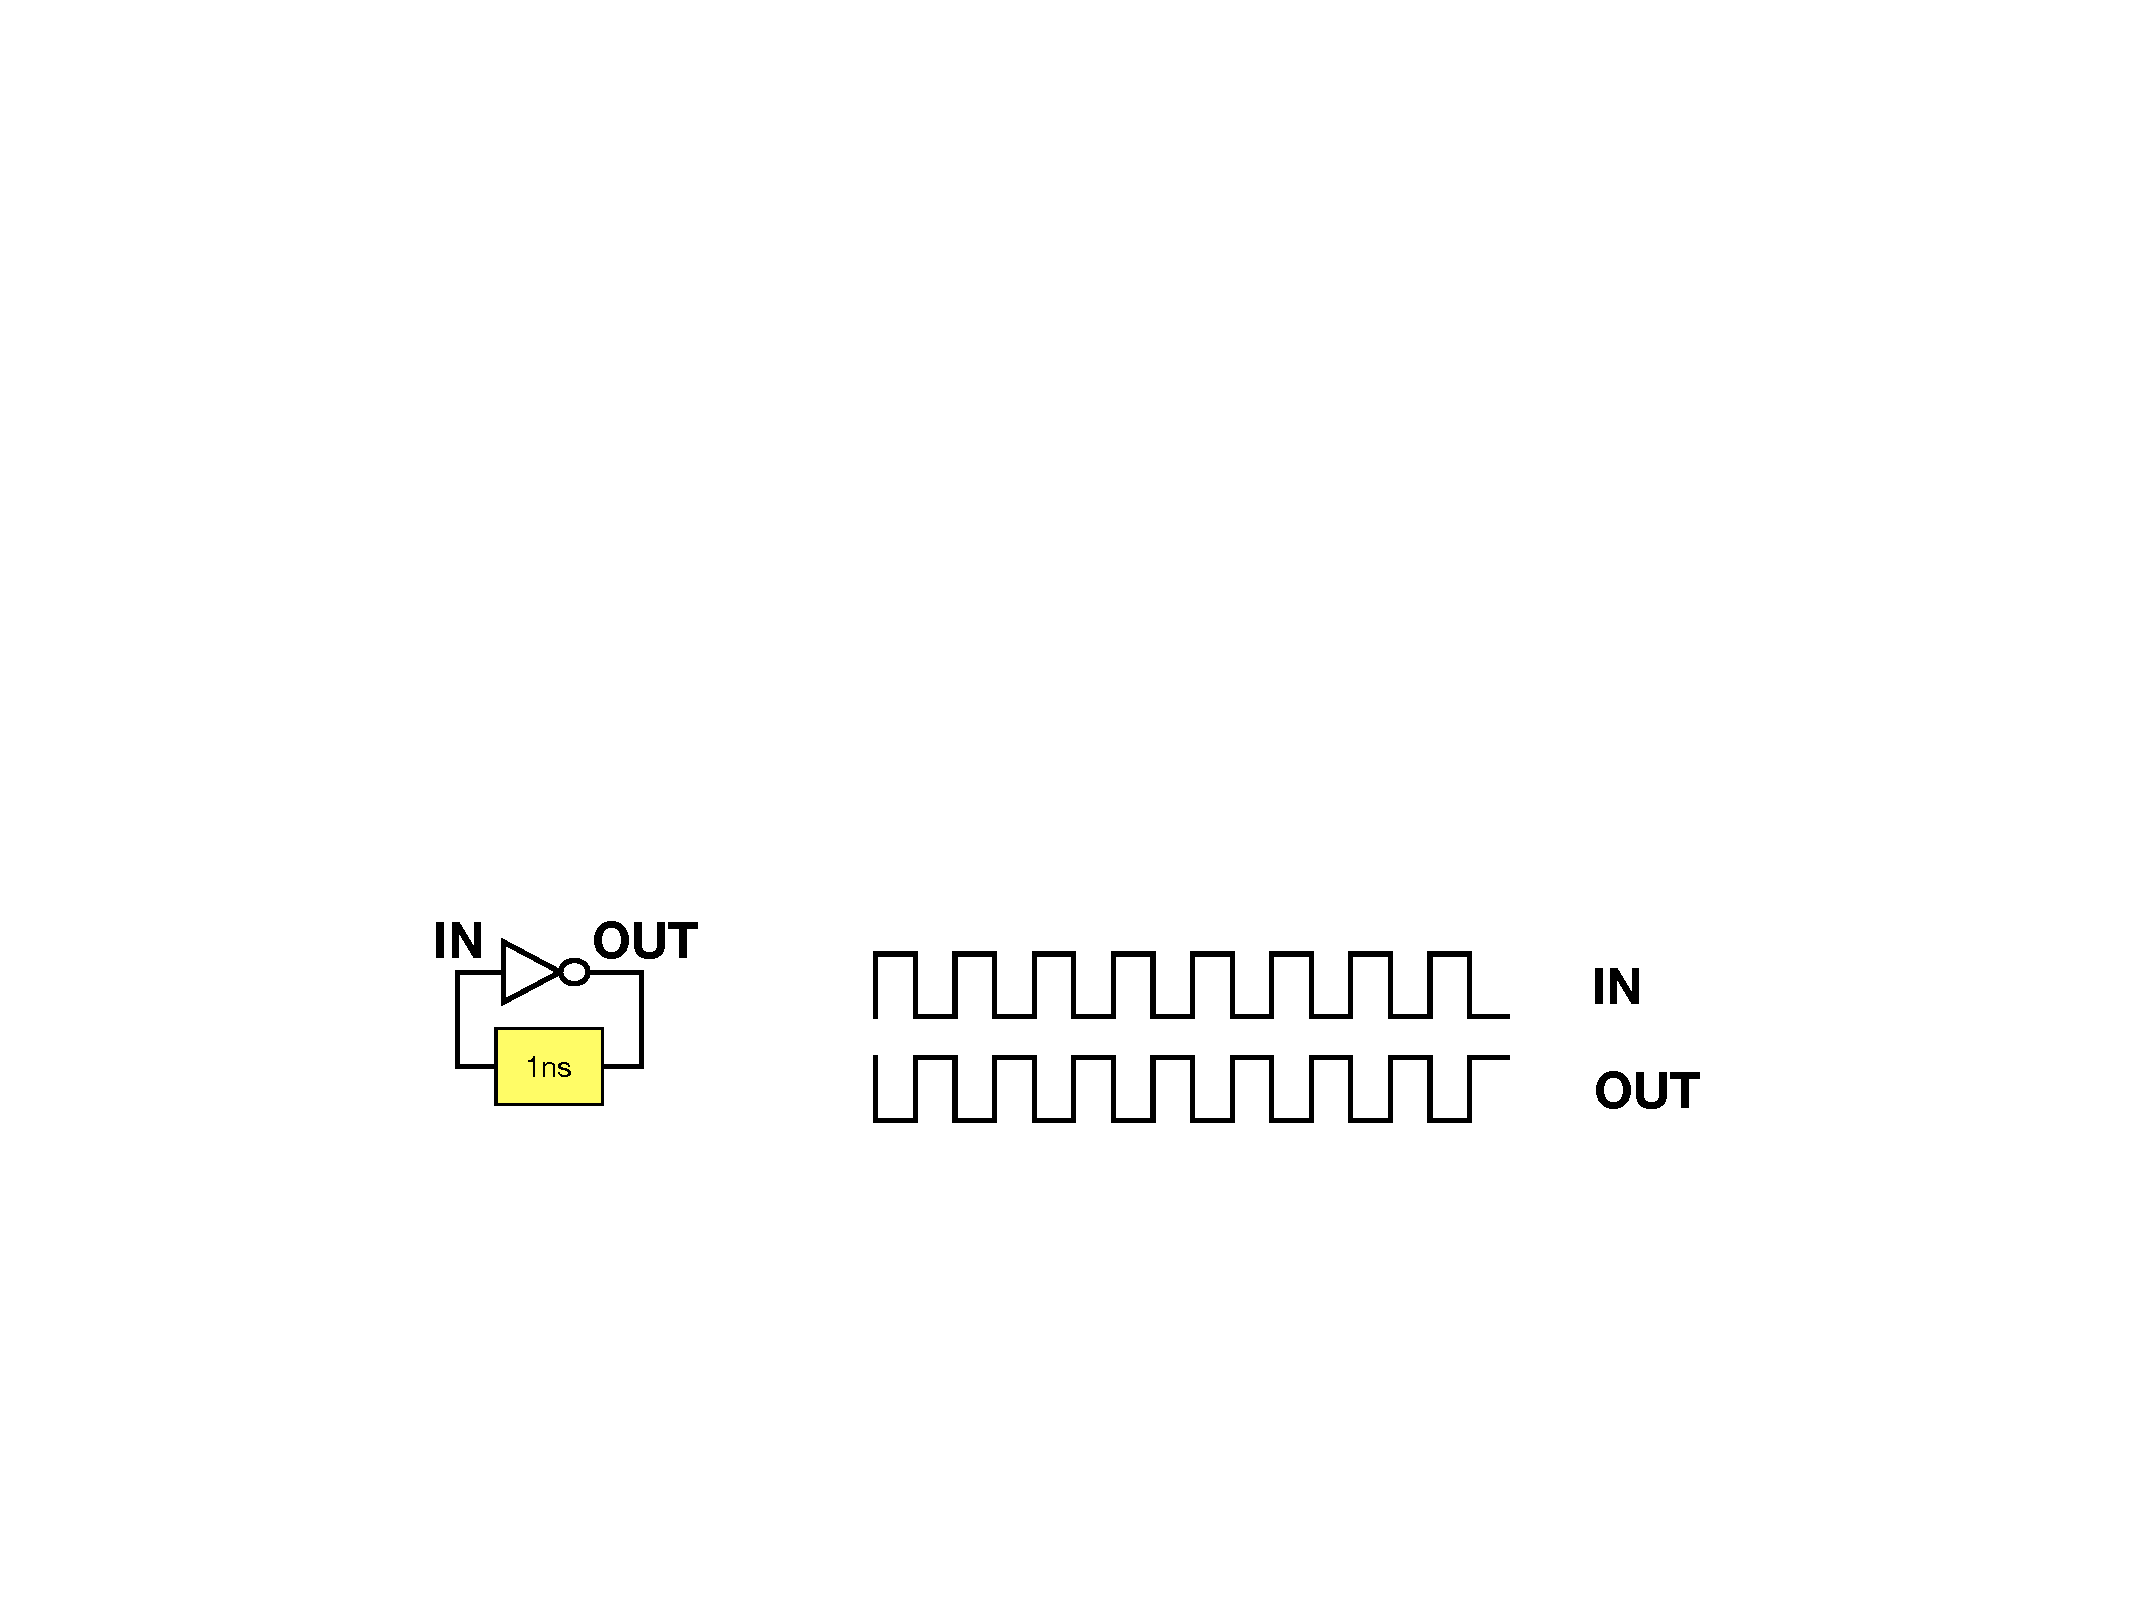
\includegraphics[width=0.5\textwidth]
    {chapter_3/figures/oscillator_logic.pdf}
    \caption{An oscillator made from a not gate and a time delay.}
    \label{fig:oscillator_logic}
\end{figure}

All oscillators can be modelled as closed loops with waves travelling around them satisfying Nyquist's criterion, which is that if you break the loop and inject an periodic signal into the broken end in a
forwards direction, if the signal arriving at the other broken end behind you with the same phase and amplitude as the injected signal, then the circuit, when reconnected, will support that oscillation indefinitely. In this case it works because the $\rm 1\,ns$ delay is half a period, so it flips the sign of the square wave, and the not
gate flips it back again, so the round trip phase shift is a full
cycle.

Oscillators are going to play an important role in digital circuits, 
but they are difficult to fabricate on conventional semiconductor
wafers, so commonly the oscillator is an external device mounted
next to the digital processor, such as a crystal or MEMs oscillator. These cost litle and have a frequency stability of tens of
parts per million. If you need a far more stable oscillator,
commercial reference oscillators based on atomic transitions in
caesium or rubidium routinely achieve frequency stabilities of
parts in $10^{11}$. Intermediate performance is achieved by
quartz oscillators phase locked to the 1 pulse-per-second 
carrier transmitted by the GPS satellite system. Digital signal
processing circuits like FPGAs also often incorporate phase locked
loops, which can generate an internal square wave oscillator on the
chip which is phase locked to the internal reference, even if the 
required frequency isn't the same as that of the reference. 

\section{Registers}
\label{sec:registers}

The value of oscillators is that they enable timing of processes, because the regular oscillation of an incoming square wave from the oscillator can be used to drive a counter. However, counters require some form of memory to store the current value that the count has reached. Logic gates cannot be made to store anything on their own, so a new type of component is needed. The simplest form of storage available in a logic circuit is a register, or bank of registers, which can store a binary number for some defined period of time. The hardware circuit that enables registers to store information on an FPGA is called a D flip-flop. 

A diagram of a D flip-flop is shown in Figure
\ref{fig:dflipflop}.

\begin{figure}[htbp]
    \centering
    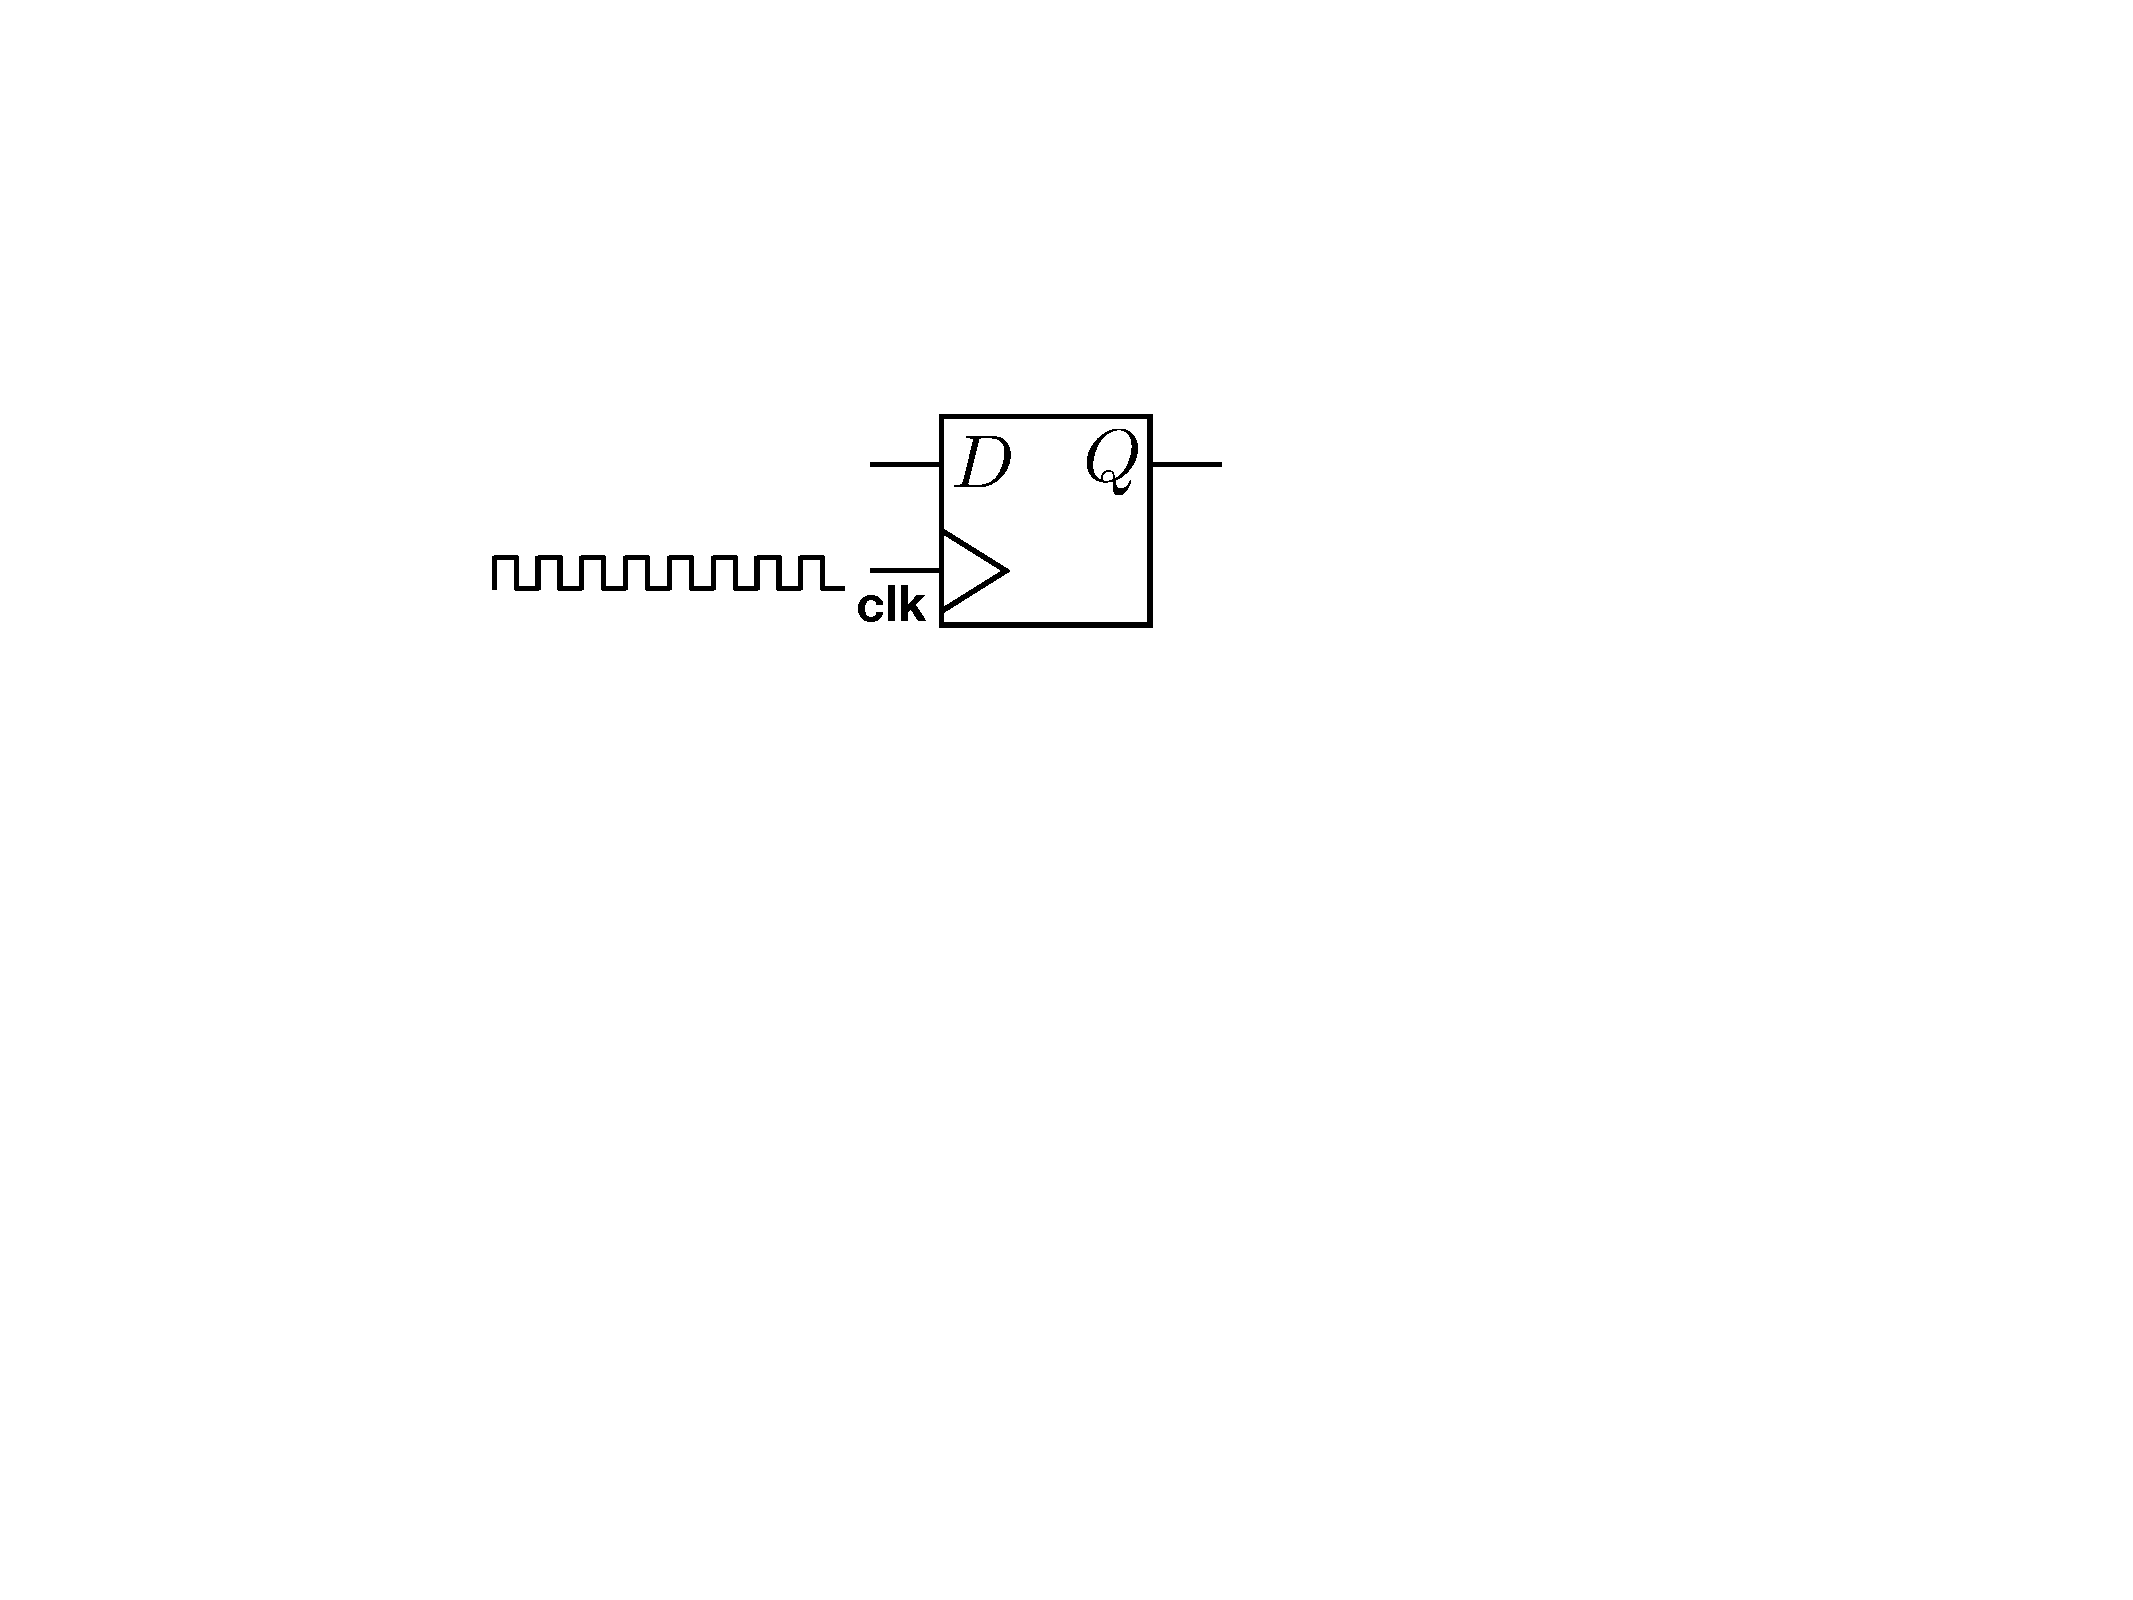
\includegraphics[width=0.5\textwidth]{figures/d_flip_flop_open.pdf}
    \caption{Standard schematic representation of a  D flip-flop circuit.}
    \label{fig:dflipflop}
\end{figure}

The flip-flop has three ports, two input and one output. One of the input ports is dedicated to an oscillator input signal. Often these signals are referred to as clocks, and \texttt{clk} will often be the name of the incoming signal, but really it is just a square wave oscillator. The other input signal I will call D, and the output signal is Q. For now let us think of D and Q as single bit signals. If we wish to store more than one bit, a bank of D flip-flops is connected in parallel to the same oscillator, and one flip-flop handles each bit.

The function of the flip-flop can be thought of classically as follows. When the rising edge of the oscillator input is detected, the digital signal present at $D$ at that time is copied to $Q$, where it remains persistent until the next rising edge of the clock input, when the cycle repeats. The process of reading the signal at $D$ and setting the $Q$ output equal to that signal is called a register transfer. Because the signal is held at the Q output for a clock period, this provides a storage mechanism for digital data.



\end{document}
